\documentclass[a4paper,12pt]{report}
%general packages
\usepackage[T2A]{fontenc}
\usepackage[utf8]{inputenc}
\usepackage[english,russian]{babel}
\usepackage{circuitikz}
\usepackage{wrapfig}
\usepackage{makecell}
\usepackage{tabularx}
\usepackage{graphicx}
\usepackage{gensymb}
\usepackage{cancel} %cancel symbol
\usepackage{amsmath,amsfonts,amssymb,amsthm,mathtools}
\usepackage[dvipsnames]{xcolor}


%\usepackage{epstopdf} %converting to PDF
%\usepackage{auto-pst-pdf}

%fancy header + geometry
\usepackage{fancyhdr}
\usepackage[a4paper,includehead,nomarginpar,left=15mm,right=15mm,top=15mm,headheight=10mm,bottom=20mm]{geometry}

%pgfplots
\usepackage{pgfplots}
\usepackage{pgfkeys}
\pgfplotsset{compat=1.12}
\usepackage{mathrsfs}

%multi column text
\usepackage{blindtext}
\usepackage{multicol}

%tikz (draw)
\usepackage{tikz}
\usepackage{pstricks-add}
\usetikzlibrary{intersections}
\usetikzlibrary{arrows.meta}
\usetikzlibrary{calc,angles,positioning}
\usetikzlibrary{arrows}
\usepackage{float}
\usepackage{filecontents}

%parskip settings
\parindent=0ex
\setlength{\parskip}{\baselineskip}%
\setlength{\parindent}{0pt}%

%fancy notation for sets
\newcommand{\R}{{\mathbb R}}
\newcommand{\N}{{\mathbb N}}
\newcommand{\fancy}[1]{{\mathbb{#1}}}
%sgn function
\DeclareMathOperator{\sgn}{sgn}

% intersection and union symbols
\newcommand{\uni}{\cup}
\newcommand{\inter}{\cap}
\newcommand{\re}{\text{Re}}
\newcommand{\const}{\text{const}}

\renewcommand{\footrulewidth}{0.4pt}

%\newcommand{\celsius}{$\ ^\circ C$}

%environments

\newtheorem{problem}{Задача}[]
\newenvironment{sol}{\paragraph{Решение}}{}
\renewcommand\thesection{\arabic{section}}

\usepackage{titlesec}
\titlespacing*{\section}
{0cm}{\baselineskip}{0pt}
\titlespacing*{\subsection}
{0pt}{0.1\baselineskip}{0.1\baselineskip}
\titlespacing*{\paragraph}
{0pt}{0.1\baselineskip}{\baselineskip}

\setcounter{secnumdepth}{0}

\begin{document}
	

\begin{titlepage}
	\begin{center}
		МОСКОВСКИЙ ФИЗИКО-ТЕХНИЧЕСКИЙ ИНСТИТУТ (НАЦИОНАЛЬНЫЙ ИССЛЕДОВАТЕЛЬСКИЙ УНИВЕРСИТЕТ) \\
		
		
		\hfill \break
		Факультет обшей и прикладной физики\\
		\vspace{2.5cm}
		\large{\textbf{Отчёт по лабораторной работе 1.2.5 <<Исследование прецессии уравновешенного гороскопа>>}}\\
		\hfill \break
		\\
	\end{center}
	
	\begin{flushright}
		Выполнил:\\
		Студент гр. Б02-304\\
		Головинов. Г.А.
	\end{flushright}
	
	\vspace{7cm}
	
	\begin{center}
		
\includegraphics[width=0.15\linewidth]{uni}
	\end{center}
	

	

	\vfill
	
	\begin{center} Долгопрудный, 2023 \end{center}
	
	\thispagestyle{empty}
	
\end{titlepage}


	\newpage
	%\pagenumbering{arabic}
    \pagestyle{fancy}

    \fancyhead{}
    \fancyfoot{}
    \fancyhead[L]{\rightmark}
    \fancyhead[R]{\thepage}
    \fancyfoot[R]{Работа 2.4.1. --- определение теплоты испарения жидкости}

    \section*{Аннотация}
        \paragraph*{Цель работы:} 1) измерить давление насыщенного пара жидкости при разной температуре; 2) вычислить по полученным данным теплоты испарения с помощью уравнения Клапейрона---Клаузиуса.
        \paragraph*{В работе используются:} термостат, герметичный сосуд, исследуемая жидкости, отсчетный микроскоп. 
    \vspace{0.5cm}
    \hrule

    \section{Основные теоретические сведения}


    \begin{multicols}{2}

    Получим условие равновесия двух фаз:

    Пусть $N_1, N_2$ --- количество частиц в фазах 1 и 2, а $V_1, V_2$ --- объемы, тогда
    \begin{equation}
        \label{dN}
        dN_1=-dN_2, \quad dV_1=-dV_2
    \end{equation}
    Запишем для обеих фаз изменение внутренней энергии:
    \begin{gather*}
        dU_1=TdS_1-pdV_1+\mu_1 dN_1 \\
        dU_2=TdS_2-pdV_2+\mu_1 dN_2
    \end{gather*}
    сложим предыдущие равенства и получим слева ноль в силу изолированности системы.
    \begin{equation*}
        T(dS_1+dS_2)-p(dV_1+dV_2)+\mu_1 dN_1 + \mu_2 dV_2 = 0
    \end{equation*}
    в силу \eqref{dN} получим
    \begin{equation*}
        T(dS_1+dS_2)=(\mu_1-\mu_2)dV_2
    \end{equation*}
    в равновесии энтропия максимальна, значит $dS_1+dS_2=0$, отсюда получим условие равновесия двух фаз:
    \begin{equation}
        \label{condition}
        \mu_1(p,T)=\mu_2(p_T)
    \end{equation}
    Теперь можно расписать изменение химических потенциалов:
    \begin{gather*}
        d\mu_1=-s_1dT+v_1dp
        d\mu_2=-s_2dT+v_2dp
    \end{gather*}
    Вследствие равенства самих потенциалов равны и их изменения:
    \begin{equation*}
        (s_2-s_1)dT=(v_2-v_1)dp
    \end{equation*}
    Отсюда получается соотношение Клапейрона---Клаузиуса:
    \begin{equation}
        \frac{dp}{dT}=\frac{s_2-s_1}{v_2-v_1}\cdot\frac{T}{T}=\frac{q}{T(v_2-v_1)}
    \end{equation}
    где $q$ --- удельная теплота фазового перехода при переходе из состояния 1 в состояние 2 (при испарении положительна, при конденсации отрицательна), $v_1, v_2$ --- удельные объемы в соответствующих состояниях.

    Для нашей работы актуальна следующая версия этого соотношения:
    \begin{equation}
        \label{clausius}
        \frac{dp}{dT}=\frac{L}{T(V_2-V_1)}
    \end{equation}
    где $p$ --- давление насыщенного пара при температуре $T$ --- абсолютная температура жидкости и пара, $L$ --- теплота испарения жидкости, $V_2$ --- объем пара, $V_1$ --- объем жидкости. Все величины относятся к одному молю вещества.

    Объем жидкости $V_1$ намного меньше чем объем пара $V_2$ (менее 0.5\% от $V_2$). Поэтому $V_1$ можно пренебречь.

    Объем $V_2$ теперь будем просто обозначать $V$. Его можно связать с давлением и температурой уравнением Ван-дер-Ваальса:
    \begin{equation}
        \label{vdv}
        \left(p+\frac{a}{V^2}\right)(V-b)=RT
    \end{equation}
    табличная величина $b$ тоже достаточно мала (соизмерима с $V_1$, которым мы пренебрегли), поэтому и ее мы учитывать не будем.
    
    Пренебрежение $a/V^2$ дает ошибку менее 3\%, при давлении ниже атмосферного ошибка становится еще меньше. Таким образом, будем считать насыщенный пар идеальным газом:
    \begin{equation}
        \label{ideal}
        pV=RT
    \end{equation}
    Подставляя \eqref{ideal} в \eqref{clausius} получим:
    \begin{equation}
        \label{L}
        L=\frac{RT^2}{p}\cdot\frac{dp}{dT}=-R\frac{d(\ln p)}{d(1/T)}
    \end{equation}
    \end{multicols}

    \hrule

    \section{Экспериментальная установка}
    \begin{figure}[H]
        \centering
        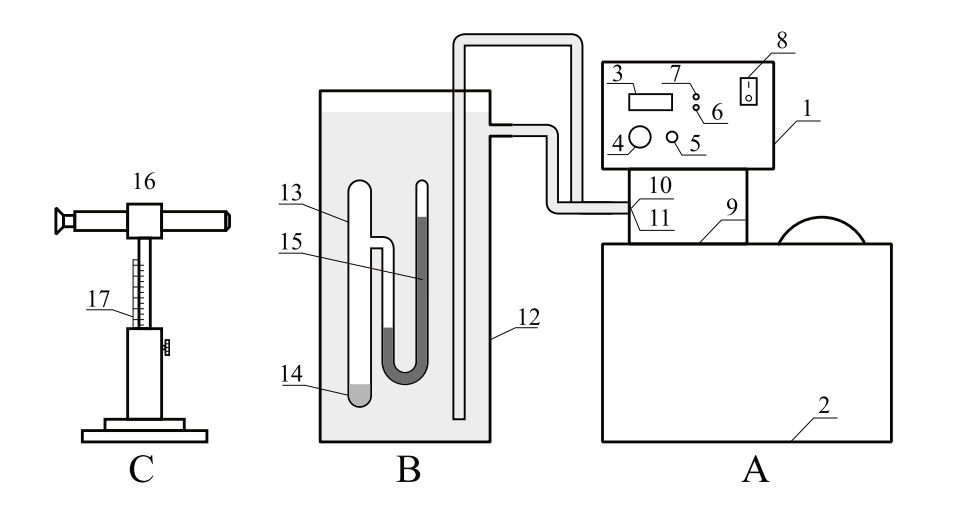
\includegraphics[width=0.9\columnwidth]{../img/experiment.png}
        \caption{Схема установки для определения теплоты испарения}
    \end{figure}
    Температура выставляется с помощью термостата А, давление измеряется при помощи экспериментального прибора B и микроскопа C: оно определяется с помощью ртутного манометра 15. Высоту столба (разницы столбов) мы измеряем с помощью микроскопа 16 и шкалы 17. 

    \section{Обработка полученных результатов}

    \begin{figure}[H]
        \centering
        \begin{tikzpicture}[]
            \begin{axis}[
                width=0.65\linewidth,
                name=plot1,
                ymajorgrids=true,
                xmajorgrids=true,
                title={$\ln{p}(1/T)$},
                xlabel={$1/T, \ \text{K}^{-1}$},
                ylabel={$\ln{p}$},
                legend pos = south west,
                legend style={nodes={scale=1, transform shape}}, 
                %legend image post style={mark=*},
            ]
            \addplot[
                only marks,mark=*,color=red,mark size = 1pt
            ]
            plot [error bars/.cd, y dir = both, x dir = both, y explicit, x explicit]
            table[meta=label, x=1/t, y=lnp, x error = et, y error = ep]{
                1/t	lnp	et	ep	label
0.003376553	8.696982308	2.85028E-06	0.022276676	1
0.00336519	8.768748489	2.83113E-06	0.020733983	1
0.003354354	8.835513433	2.81292E-06	0.01939488	1
0.00334314	8.897004744	2.79415E-06	0.018238191	1
0.00333189	8.959226614	2.77537E-06	0.017137961	1
0.003320825	9.012941994	2.75697E-06	0.016241676	1
0.003309834	9.074206524	2.73875E-06	0.015276505	1
0.003298697	9.131212161	2.72035E-06	0.014430014	1
0.003287851	9.191412281	2.70249E-06	0.013586957	1
0.003276969	9.241366363	2.68463E-06	0.012924906	1
0.003266266	9.303624271	2.66712E-06	0.012144766	1
0.00325595	9.357064882	2.6503E-06	0.011512779	1
0.003234676	9.464484065	2.61578E-06	0.010340192	1
0.003213368	9.568861779	2.58143E-06	0.009315324	1
0.003198362	9.632118622	2.55738E-06	0.008744316	1

            };
            \addlegendentry[]{Нагревание}
            \addplot[
                only marks,mark=*,color=blue,mark size = 1pt
            ]
            plot [error bars/.cd, y dir = both, x dir = both, y explicit, x explicit]
            table[meta=label, x=1/t, y=lnp, x error = et, y error = ep]
            {
                1/t	lnp	et	ep	label
0.003215848	9.5670903	2.58542E-06	0.00933184	1
0.003226223	9.530114173	2.60213E-06	0.009683354	1
0.003236979	9.475794076	2.61951E-06	0.010223903	1
0.003247175	9.423321647	2.63604E-06	0.010774701	1
0.003257753	9.368170383	2.65324E-06	0.011385631	1
0.003267333	9.302044204	2.66887E-06	0.01216397	1
0.003279011	9.250373115	2.68798E-06	0.012809018	1
0.003288825	9.191819806	2.70409E-06	0.013581421	1
0.003300003	9.138544521	2.72251E-06	0.014324595	1
0.003311039	9.095966222	2.74074E-06	0.014947683	1
0.003322259	9.030171307	2.75935E-06	0.01596424	1
0.003332778	8.983605678	2.77685E-06	0.016725205	1
0.003343587	8.903730208	2.79489E-06	0.018115942	1
0.003355254	8.853008833	2.81443E-06	0.01905851	1
0.00336621	8.768541128	2.83284E-06	0.020738283	1
0.003377351	8.720756265	2.85163E-06	0.021753317	1

            };
            \addlegendentry{Охлаждение}
            \addplot[red,dashed,domain=0.00319:0.00339] {-5160.29*x+26.15};
            \addlegendentry{Аппроксимация нагревания}
            \addplot[blue,dashed,domain=0.00319:0.00339] {-5239.06*x+26.43};
            \addlegendentry{Аппроксимация охлаждения}
        \end{axis}
    \end{tikzpicture}
\end{figure}

\begin{multicols}{2}
    С помощью метода $\chi^2$ получены две прямые:

    \begin{gather*}
        \ln{p}=-5160.3\cdot \frac{1}{T} + 26.2 \\
        \ln{p}=-5239.1\cdot \frac{1}{T} + 26.2
    \end{gather*}

    первая --- для нагревания, вторая --- для охлаждения. (Погрешности получились около 3-го знака после запятой, поэтому ими можно пренебречь).

    Видно, что прямые несколько отличаются, однако относительная разница коэффициентов $k$ наклона прямых около $1.5\%$.

    Погрешности оцениваем следующим образом:

    \begin{gather*}
        \sigma\left(1/T\right)=1/T \cdot \varepsilon_T\\
        \sigma(\ln p)=\varepsilon_p
    \end{gather*}

    Вычисляем по формуле \eqref{L} значения теплоты испарения спирта:

    \begin{gather*}
        L_\text{нагревания}=42.9\pm 2.1\  \text{кДж/моль}\\
        L_\text{охлаждения}=43.5\pm 2.2\  \text{кДж/моль}
    \end{gather*}

    Погрешность $L$ взята за 5\%, берется из пренебрежения $a$ и $b$.

    Переведем в СИ и получим:
    \begin{gather*}
        L_\text{нагревания}=932.6\pm 46.6 \ \text{кДж/кг}\\
        L_\text{охлаждения}=945.6\pm 47.3 \ \text{кДж/кг}
    \end{gather*}

    Полученные значения попадают в интервал $\pm 2\sigma$, что говорит о недооценке погрешности и несовершенстве используемой модели.
\end{multicols}

\newpage
\section{Выводы}
\begin{multicols}{2}
    В результате работы были получены значения удельной теплоты парообразования спирта в двух случаях: при нагревании и при охлаждении. Полученные значения немного отличаются от табличных, однако попадают в интервал $\pm 2\sigma$, что говорит о недооценке погрешности и несовершенстве модели.
\end{multicols}

\section{Приложение}
\begin{multicols}{2}
    \begin{table}[H]
        \centering
        \begin{tabular}{|c|c|c|c|}
            \hline
            $1/T, \ \text{K}^{-1}$ & $\ln p$ & $\sigma_{1/T}, \ \text{K}^{-1}$ & $\sigma_{\ln p}$ \\
            \hline
            0.0034 & 8.697 & 2.85E-06 & 0.022 \\
            \hline
            0.0034 & 8.769 & 2.83E-06 & 0.021 \\
            \hline
            0.0034 & 8.836 & 2.81E-06 & 0.019 \\
            \hline
            0.0033 & 8.897 & 2.79E-06 & 0.018 \\
            \hline
            0.0033 & 8.959 & 2.78E-06 & 0.017 \\
            \hline
            0.0033 & 9.013 & 2.76E-06 & 0.016 \\
            \hline
            0.0033 & 9.074 & 2.74E-06 & 0.015 \\
            \hline
            0.0033 & 9.131 & 2.72E-06 & 0.014 \\
            \hline
            0.0033 & 9.191 & 2.70E-06 & 0.014 \\
            \hline
            0.0033 & 9.241 & 2.68E-06 & 0.013 \\
            \hline
            0.0033 & 9.304 & 2.67E-06 & 0.012 \\
            \hline
            0.0033 & 9.357 & 2.65E-06 & 0.012 \\
            \hline
            0.0032 & 9.464 & 2.62E-06 & 0.010 \\
            \hline
            0.0032 & 9.569 & 2.58E-06 & 0.009 \\
            \hline
            0.0032 & 9.632 & 2.56E-06 & 0.009 \\
            \hline
        \end{tabular}
        \caption{Результаты измерений для нагревания}
    \end{table}
    \newcolumn

    \begin{table}[H]
        \centering
        \begin{tabular}{|c|c|c|c|}
            \hline
            $1/T, \ \text{K}^{-1}$ & $\ln p$ & $\sigma_{1/T}, \ \text{K}^{-1}$ & $\sigma_{\ln p}$ \\
            \hline
            0.0032 & 9.567 & 2.59E-06 & 0.009 \\
            \hline
            0.0032 & 9.530 & 2.60E-06 & 0.010 \\
            \hline
            0.0032 & 9.476 & 2.62E-06 & 0.010 \\
            \hline
            0.0032 & 9.423 & 2.64E-06 & 0.011 \\
            \hline
            0.0033 & 9.368 & 2.65E-06 & 0.011 \\
            \hline
            0.0033 & 9.302 & 2.67E-06 & 0.012 \\
            \hline
            0.0033 & 9.250 & 2.69E-06 & 0.013 \\
            \hline
            0.0033 & 9.192 & 2.70E-06 & 0.014 \\
            \hline
            0.0033 & 9.139 & 2.72E-06 & 0.014 \\
            \hline
            0.0033 & 9.096 & 2.74E-06 & 0.015 \\
            \hline
            0.0033 & 9.030 & 2.76E-06 & 0.016 \\
            \hline
            0.0033 & 8.984 & 2.78E-06 & 0.017 \\
            \hline
            0.0033 & 8.904 & 2.79E-06 & 0.018 \\
            \hline
            0.0034 & 8.853 & 2.81E-06 & 0.019 \\
            \hline
            0.0034 & 8.769 & 2.83E-06 & 0.021 \\
            \hline
            0.0034 & 8.721 & 2.85E-06 & 0.022 \\
            \hline
        \end{tabular}
        \caption{Результаты измерений для охлаждения}
    \end{table}
\end{multicols}
\end{document}
